Dieses Experiment schränkt den Platz der Agenten weiter ein. Die Zahl der belegten Felder ist hier größer als die Anzahl der freien Felder. Besonders für dieses Experiment ist, dass ein Graph vorliegt der die Prioritätswerte der Agenten über die Zeit zeigt (siehe Abbildung \ref{tab:resultsCoDy} und \ref{tab:myResults}). 

\textbf{Aufbau des Experiments}
\begin{figure}[H]
    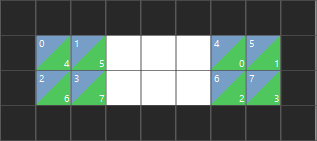
\includegraphics[height=32mm]{images/4vs4_tight.png}
    \centering
    \caption{Aufbau für die enge Vorbeifahrt zweier Gruppen, bestehend aus jeweils vier Agenten}
    \label{fig:4x4}
\end{figure}
Die Karte für dieses Experiment misst sieben mal zwei Felder. Acht Agenten teilen sich in zwei gleich große Gruppen und stehen sich gegenüber.